\section{Présentation du projet}
\subsection{Intitulé}
 L'objectif de ce projet est de développer un outil permettant à un administrateur réseau de définir à distance à partir d'un client Web, des routes\footnote{route BGP \cite{BGP}} menant vers des trous noirs pour dévier des attaques réseaux.Ces routes seront envoyées à un serveur de route qui les diffusera auprès de tous les serveurs BGP du domaine. Le logiciel devra être implémenté en Javascript et du côté serveur il devra piloter le logiciel ExaBGP écrit en Python. L'application Web devra être de type RESTful et elle s'appuiera éventuellement sur un framework JS. Elle devra supporter le routage vers trou noir par la destination, par la source et par la communauté BGP.

\subsubsection{Définitions}

Les \textbf{routes} sont définit par une adresse IP de destination, d'une adresse IP du prochain routeur (\underline{NextHop}) puis une liste des Systèmes Autonomes traversé (AS).
\\
\\
Une \textbf{Communauté} est un système Autonomes:\\
\textit{"Un Système Autonomes est un ensemble cohérent de réseaux et de routeurs sous la responsabilité d'une autorité administrative \footnote{Définition AS:  \url{http://www.linux-france.org/prj/edu/archinet/systeme/ch65s02.html}}."}
\\
\\
\textbf{Un routeur BGP}\footnote{BGP \url{https://www.cisco.com/c/en/us/support/docs/ip/border-gateway-protocol-bgp/26634-bgp-toc.html}} est un routeur qui utilise le protocole BGP (Border Gateway Protocol). BGP s'appuie sur le protocole TCP, sur le port 179. Lorsque deux routeurs BGP forment une connexion TCP entre eux. Ces routeurs sont des routeurs homologues (voisins). 
\\
\\
BGP est un protocole de type " Path Vector ". Les routeurs s'échangent des informations du type :
\\
\fbox{
\textbf{\scriptsize Adresse IP du réseau de destination}
} |
\fbox{
\textbf{\scriptsize Adresse IP du prochain routeur(next hop)}
} |
\fbox{
\textbf{\scriptsize Liste des AS traversés pour atteindre le réseau}
}
\\
\\
\textbf{Annoncer une route} :
\newline
Les routeurs qui forment une connexion TCP afin d'échanger les données de routage BGP, sont des paires('peers') ou voisins('neighbors'). Les BGP 'peers' partagent alors les informations de routage BGP(Table de routage).\newline
Normalement,  BGP 'peers' mettent à jour leurs table de routage en utilisant la technique \textbf{UPDATE Message}, cela garantit que tous les BGPs aient la même version de la table de routage, et donc le numéro de version change pour tout changement effectué auprès n'importe quel 'peer'.

\pagebreak
\textbf{Next-Hop}\cite{Routing_BGP} : Cette terme désigne l'adresse IP du prochain routeur auquel le paquet IP devrait être transmis afin que ce paquet IP puisse atteindre sa destination.
\newline
Afin d'illustrer le fonctionnement de l'attribut Next Hop, nous détaillons ce dernier sur un exemple :  
\newline
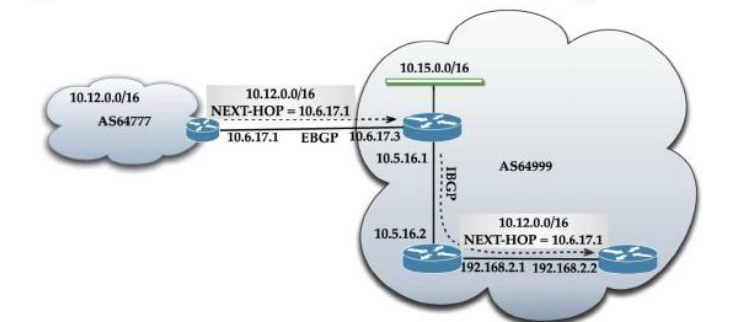
\includegraphics[scale = 0.5]{img/nextHope.jpg}
\\
\\
  Dans ce scénario, si la destination qu'on souhaite atteindre est le réseau : "10.12.0.0/16", donc, tout trafic allant à cette adresse, doit s'orienter vers le routeur "10.6.17.1". Cela veut dire que le prochain routeur (Next-Hop) du "10.12.0.0/16" est le "10.6.17.1".
\newline
L'adresse 10.12.0.0/16 est annoncé par le EBGP (External BGP) 10.6.17.1, et donc l'information est passé de la communauté "AS64777" à la "AS649999". Ensuite le UPDATE Message est passé aux voisins par le iBGP(internal BGP) afin que tous les BGP peers gardent la même version de la table de routage. 
% \textbf{RESTful} : 
% \\
% \\

\subsection{Le routage vers trou noir \cite{Cisco}} 

La déviation des routes vers un trou noir, aussi appelée "Remotely-Triggered Black Hole (RTBH)" en anglais, est une technique qui permet de faire tomber (suspendre) un trafic provenant d'une source étant indésirable, avant que ce dernier puisse entrer dans un réseau protégé.
\\
\\
Le routage vers trou noir est essentiellement utilisé pour défendre ou proprement dit pour atténuer les attaques DDoS (distributed-denial-of-service). Les trous noirs sont placés principalement dans un réseau pour lequel, on peut dévier et/ou suspendre le trafic lorsque le système détecte une attaque. 
\newline
Pour que le système puisse dévier des router, il se base sur l'adresse IP de la destination ou bien de l'adresse IP source. Donc, il existe deux méthodologies :
\\
\begin{itemize}
\item \textbf{Destination-Based Remotely Triggered Black Hole Filtering } : On rend l'adresse IP de la destination inaccessible, en déviant toutes les routes allant à cet adresse vers le trou noir.
\item \textbf{Source-Based Remotely Triggered Black Hole Filtering }
: Dans ce scénario, si le trafic provenant d'une adresse IP est susceptible d'être une attaque, alors, tout trafic lié à cet adresse IP serait suspendu. Cela veut dire que selon l'adresse source IP, cette dernière ne peut pas avoir accès à sa destination. En outre, on fait tomber tous les chemins partants d'une adresse IP source précise.   
\end{itemize}


